\section{An initial overview of power electronics}
%\part{An initial overview of power electronics}
\title[Initial overview]{An initial overview of power electronics}  

\begin{frame}[plain]
    \titlepage
\end{frame}


%%%%%%%%%%%%%%%%%%%%%%%%%%%%%%%%%%%%%%%%%%%%%%%%%%%%%%%%%%%%%
%% What are power electronics? %%
%%%%%%%%%%%%%%%%%%%%%%%%%%%%%%%%%%%%%%%%%%%%%%%%%%%%%%%%%%%%%
\begin{frame}
	\frametitle{What are power electronics?}
		\vspace{0.5cm}
		\begin{figure}
		\begin{tikzpicture}[auto, node distance=1cm and 2cm]
			\draw
				node [input, name = input] {}
				node [block, right = of input] (pc) {Power converter}
				node [block, right = of pc] (load) {Load}
				node [block, below = of pc] (controller) {Controller}
				node [input, left = of controller, name = ref] {};
			\draw [->] (input) -- node  {$u_\mathrm{in}, i_\mathrm{in}$} (pc);
			\draw [->] (pc) -- node [name=M]  {$u_\mathrm{out}, i_\mathrm{out}$} (load);
			\draw [->] (ref) -- node  {Reference} (controller);
			\draw[->] (M) |- (controller);
			\draw[->] (controller) -- node {Feedback} (pc);
			\node[dot] at (M.south) {}; 
		\end{tikzpicture}
		\caption{High-level block diagram of a power electronic system}
		\label{fig:power_electronics_block_diagram}
	\end{figure}
	\begin{varblock}[0.9\textwidth]{Power electronics -- a definition}
		Power electronics is a multidisciplinary branch of electrical engineering. It focuses on processing, controlling, and converting electric power. Power electronics manipulate voltages and currents to deliver a defined power to electrical equipment and devices.
	\end{varblock}
\end{frame}

%%%%%%%%%%%%%%%%%%%%%%%%%%%%%%%%%%%%%%%%%%%%%%%%%%%%%%%%%%%%%
%% Power electronics vs. microelectronics %%
%%%%%%%%%%%%%%%%%%%%%%%%%%%%%%%%%%%%%%%%%%%%%%%%%%%%%%%%%%%%%
\begin{frame}
	\frametitle{Power electronics vs. microelectronics}
		\vspace{0.5cm}
		\begin{figure}
		\begin{tikzpicture}[auto, node distance=1cm and 2cm]
			\matrix[column sep=0.03\textwidth, row sep=0.5cm]{
				\draw
					node [input, name = input, label=left:{Control signals}] {}
					node [block, right = of input, minimum width = 3.5cm] (pc) {Power electronics}
					node [output, right = of pc, name = output, label=right:{Output power}] {}
					node [input, above = of pc, name = control, label=above:{Control signals}] {};
				\draw [->] (input) --  (pc);
				\draw [->] (pc) -- (output);
				\draw [->] (control) -- (pc);
			\\
				\draw
					node [input, name = input, label=left:{Input signals}] {}
					node [block, right = of input, minimum width = 3.5cm] (pc) {Microelectronics}
					node [output, right = of pc, name = output, label=right:{Output signals}] {}
					node [input, below = of pc, name = control, label=below:{Power supply}] {};
				\draw [->] (input) --  (pc);
				\draw [->] (pc) -- (output);
				\draw [->] (control) -- (pc);
			\\
			};			
		\end{tikzpicture}
		\caption{Power electronics vs. microelectronics}
		\label{fig:power_electronics_vs_microelectronics}
	\end{figure}
\end{frame}


%%%%%%%%%%%%%%%%%%%%%%%%%%%%%%%%%%%%%%%%%%%%%%%%%%%%%%%%%%%%%
%% Power electronic tasks %%
%%%%%%%%%%%%%%%%%%%%%%%%%%%%%%%%%%%%%%%%%%%%%%%%%%%%%%%%%%%%%
\begin{frame}[c]
	\frametitle{Typical voltage and current manipulation tasks of power electronics}
	\begin{figure}
		\centering
		\begin{tikzpicture}[ampersand replacement=\&]
			\matrix[column sep=0.03\textwidth, row sep=0.5cm]{
			\begin{axis}[
				width=0.3\textwidth,
				height=0.4\textheight,
				axis lines=middle,
				xlabel={$\omega t$},
				ylabel={$u(\omega t)$},
				xlabel style={yshift=.0*\pgfkeysvalueof{/pgfplots/major tick length},
				anchor=west,
				inner xsep=0pt,
				xshift=0.5*\pgfkeysvalueof{/pgfplots/major tick length}},
				ylabel style={yshift=1.5*\pgfkeysvalueof{/pgfplots/major tick length},
				anchor=north west,
				inner ysep=0pt},
				xmin=0, xmax=2*pi,
				ymin=-1.5, ymax=1.5,
				xtick={0,1.57,3.14,4.71,6.28},
				xticklabels={$0$,$\frac{\pi}{2}$,$\pi$,$\frac{3\pi}{2}$,$2\pi$},
				ytick={-1,0,1},
				yticklabels={$-\hat{u}$,$0$,$\hat{u}$},
				grid=both,
				]
				\addplot[domain=0:2*pi, samples=100, signalblue, thick]{1};
			\end{axis}
			\&
			\begin{axis}[
				width=0.3\textwidth,
				height=0.4\textheight,
				axis lines=middle,
				xlabel={$\omega t$},
				ylabel={$u(\omega t)$},
				xlabel style={yshift=.0*\pgfkeysvalueof{/pgfplots/major tick length},
				anchor=west,
				inner xsep=0pt,
				xshift=0.5*\pgfkeysvalueof{/pgfplots/major tick length}},
				ylabel style={yshift=1.5*\pgfkeysvalueof{/pgfplots/major tick length},
				anchor=north west,
				inner ysep=0pt},
				xmin=0, xmax=2*pi,
				ymin=-1.5, ymax=1.5,
				xtick={0,1.57,3.14,4.71,6.28},
				xticklabels={$0$,$\frac{\pi}{2}$,$\pi$,$\frac{3\pi}{2}$,$2\pi$},
				ytick={-1,0,1},
				yticklabels={$-\hat{u}$,$0$,$\hat{u}$},
				grid=both,
				]
				\addplot[domain=0:2*pi, samples=100, signalblue, thick]{sin(deg(x))};
			\end{axis}
			\&
			\begin{axis}[
				width=0.3\textwidth,
				height=0.4\textheight,
				axis lines=middle,
				xlabel={$\omega t$},
				ylabel={$u(\omega t)$},
				xlabel style={yshift=.0*\pgfkeysvalueof{/pgfplots/major tick length},
				anchor=west,
				inner xsep=0pt,
				xshift=0.5*\pgfkeysvalueof{/pgfplots/major tick length}},
				ylabel style={yshift=1.5*\pgfkeysvalueof{/pgfplots/major tick length},
				anchor=north west,
				inner ysep=0pt},
				xmin=0, xmax=2*pi,
				ymin=-1.5, ymax=1.5,
				xtick={0,1.57,3.14,4.71,6.28},
				xticklabels={$0$,$\frac{\pi}{2}$,$\pi$,$\frac{3\pi}{2}$,$2\pi$},
				ytick={-1,0,1},
				yticklabels={$-\hat{u}$,$0$,$\hat{u}$},
				grid=both,
				]
				\addplot[domain=0:2*pi, samples=100, signalblue, thick]{sin(deg(x))};
			\end{axis}
			\\
			% add two arrows: one pointing up with a label "rectifier" and one pointing down with a label "inverter"
				\draw[->, thick] (1,0) -- (1,1);
				\node[anchor=east] at (1,0.5) {rectifier};
				\draw[->, thick] (2,1) -- (2,0);
				\node[anchor=west] at (2,0.5) {inverter};
			\&
				\draw[<->, thick] (1,0) -- (1,1);
				\node[anchor=east,  align=right] at (1,0.5) {frequency\\phase};
				\draw[<->, thick] (2,1) -- (2,0);
				\node[anchor=west] at (2,0.5) {amplitude};
			\&
				\draw[<->, thick] (1.5,0) -- (1.5,1);
				\node[anchor=east,  align=right] at (1.5,0.5) {number of\\phases};
			\\
			\begin{axis}[
				width=0.3\textwidth,
				height=0.4\textheight,
				axis lines=middle,
				xlabel={$\omega t$},
				ylabel={$u(\omega t)$},
				xlabel style={yshift=.0*\pgfkeysvalueof{/pgfplots/major tick length},
				anchor=west,
				inner xsep=0pt,
				xshift=0.5*\pgfkeysvalueof{/pgfplots/major tick length}},
				ylabel style={yshift=1.5*\pgfkeysvalueof{/pgfplots/major tick length},
				anchor=north west,
				inner ysep=0pt},
				xmin=0, xmax=2*pi,
				ymin=-1.5, ymax=1.5,
				xtick={0,1.57,3.14,4.71,6.28},
				xticklabels={$0$,$\frac{\pi}{2}$,$\pi$,$\frac{3\pi}{2}$,$2\pi$},
				ytick={-1,0,1},
				yticklabels={$-\hat{u}$,$0$,$\hat{u}$},
				grid=both,
				]
				\addplot[domain=0:2*pi, samples=100, signalblue, thick]{sin(deg(x))};
			\end{axis}
			\&
			\begin{axis}[
				width=0.3\textwidth,
				height=0.4\textheight,
				axis lines=middle,
				xlabel={$\omega t$},
				ylabel={$u(\omega t)$},
				xlabel style={yshift=.0*\pgfkeysvalueof{/pgfplots/major tick length},
				anchor=west,
				inner xsep=0pt,
				xshift=0.5*\pgfkeysvalueof{/pgfplots/major tick length}},
				ylabel style={yshift=1.5*\pgfkeysvalueof{/pgfplots/major tick length},
				anchor=north west,
				inner ysep=0pt},
				xmin=0, xmax=2*pi,
				ymin=-1.5, ymax=1.5,
				xtick={0,1.57,3.14,4.71,6.28},
				xticklabels={$0$,$\frac{\pi}{2}$,$\pi$,$\frac{3\pi}{2}$,$2\pi$},
				ytick={-1,0,1},
				yticklabels={$-\hat{u}$,$0$,$\hat{u}$},
				grid=both,
				]
				\addplot[domain=0:2*pi, samples=100, signalblue, thick]{0.5*sin(deg(2*x+pi/2))};
			\end{axis}
			\&
			\begin{axis}[
				width=0.3\textwidth,
				height=0.4\textheight,
				axis lines=middle,
				xlabel={$\omega t$},
				ylabel={$u(\omega t)$},
				xlabel style={yshift=.0*\pgfkeysvalueof{/pgfplots/major tick length},
				anchor=west,
				inner xsep=0pt,
				xshift=0.5*\pgfkeysvalueof{/pgfplots/major tick length}},
				ylabel style={yshift=1.5*\pgfkeysvalueof{/pgfplots/major tick length},
				anchor=north west,
				inner ysep=0pt},
				xmin=0, xmax=2*pi,
				ymin=-1.5, ymax=1.5,
				xtick={0,1.57,3.14,4.71,6.28},
				xticklabels={$0$,$\frac{\pi}{2}$,$\pi$,$\frac{3\pi}{2}$,$2\pi$},
				ytick={-1,0,1},
				yticklabels={$-\hat{u}$,$0$,$\hat{u}$},
				grid=both,
				]
				\addplot[domain=0:2*pi, samples=100, signalblue, thick]{sin(deg(x))};
				\addplot[domain=0:2*pi, samples=100, signalred, thick]{sin(deg(x-2*pi/3))};
				\addplot[domain=0:2*pi, samples=100, signalgreen, thick]{sin(deg(x+2*pi/3))};
			\end{axis}
			\\
			};
			% vertical arrows
			%\draw[->, thick] (0.15\textwidth,0.3\textwidth) -- (0.15\textwidth,0.7\textwidth);
			%\draw[->, thick] (0.5\textwidth,0.3\textwidth) -- (0.5\textwidth,0.7\textwidth);
		\end{tikzpicture}
	\end{figure}
\end{frame}

%%%%%%%%%%%%%%%%%%%%%%%%%%%%%%%%%%%%%%%%%%%%%%%%%%%%%%%%%%%%%
%% Power electronic application examples: residential %%
%%%%%%%%%%%%%%%%%%%%%%%%%%%%%%%%%%%%%%%%%%%%%%%%%%%%%%%%%%%%%
\begin{frame}[c]
	\frametitle{Power electronic application examples: residential}
	\begin{figure}
		\centering
		\begin{subfigure}[b]{0.49\textwidth}
			\centering
			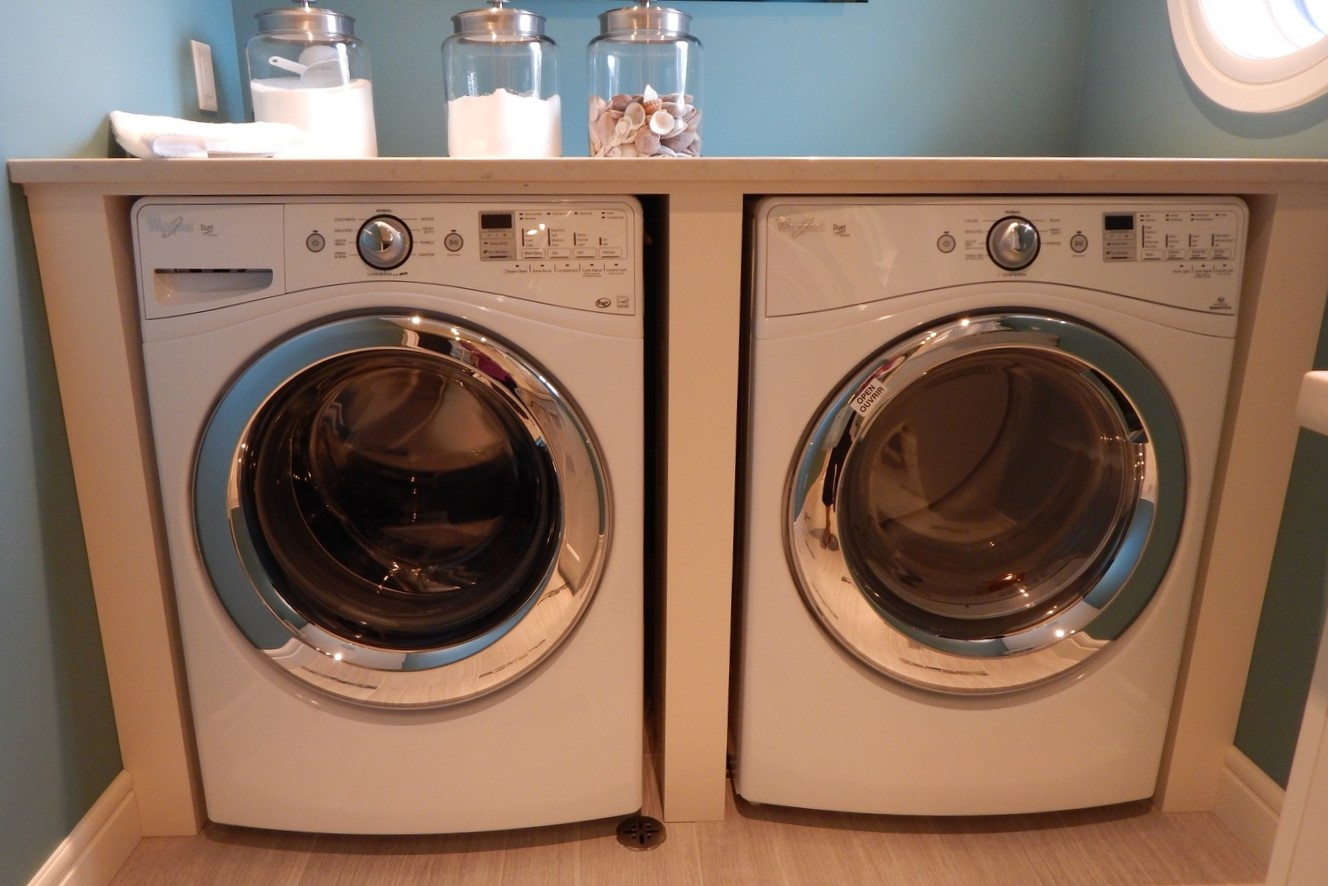
\includegraphics[width=0.5\textwidth]{fig/lec01/Home_appliance.jpg}
			\caption{Home appliances (source: \href{https://pxhere.com/de/photo/863012}{pxhere}, \href{https://creativecommons.org/publicdomain/zero/1.0/}{CC0~1.0})}
		\end{subfigure}
		\hfill
		\begin{subfigure}[b]{0.49\textwidth}
			\centering
			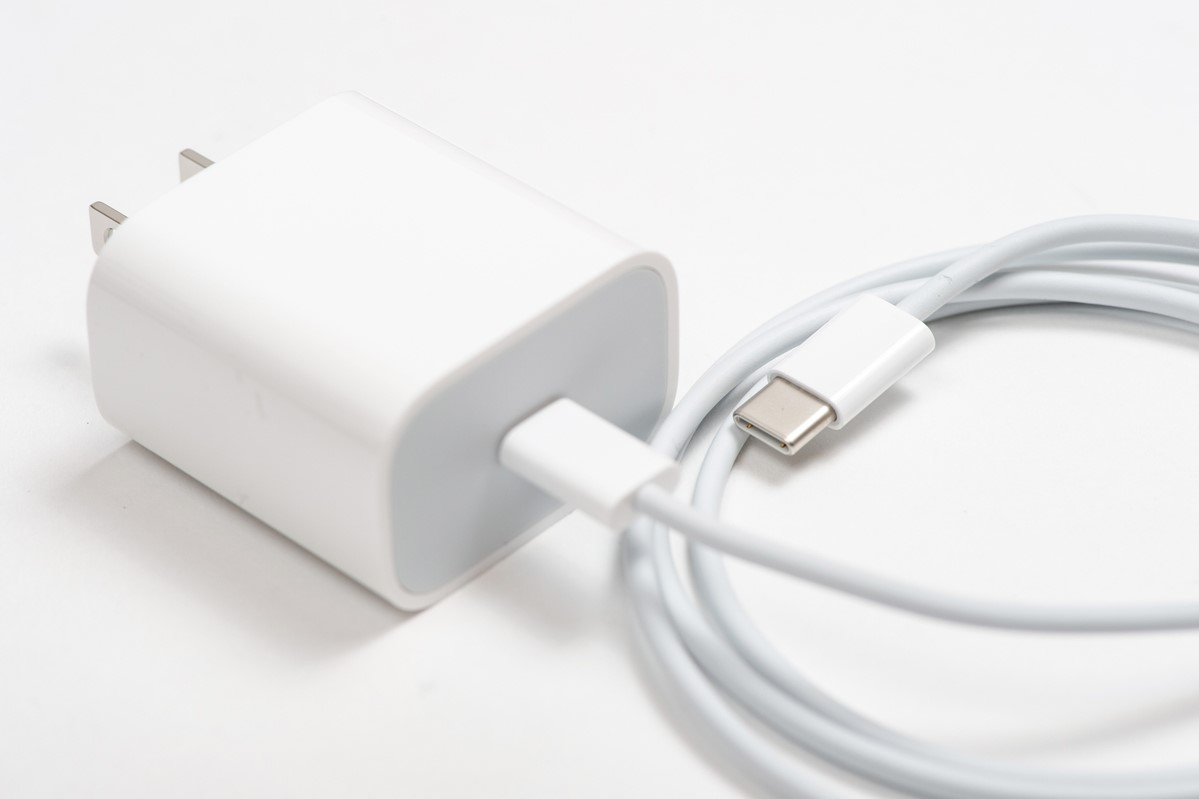
\includegraphics[width=0.5\textwidth]{fig/lec01/Smartphone_charger.jpg}
			\caption{Smartphone charger (source: \href{https://www.rawpixel.com/image/5923136/photo-image-phone-public-domain-white}{rawpixel}, \href{https://creativecommons.org/publicdomain/zero/1.0/}{CC0~1.0})}
		\end{subfigure}
		\\
		\begin{subfigure}[b]{0.49\textwidth}
			\centering
			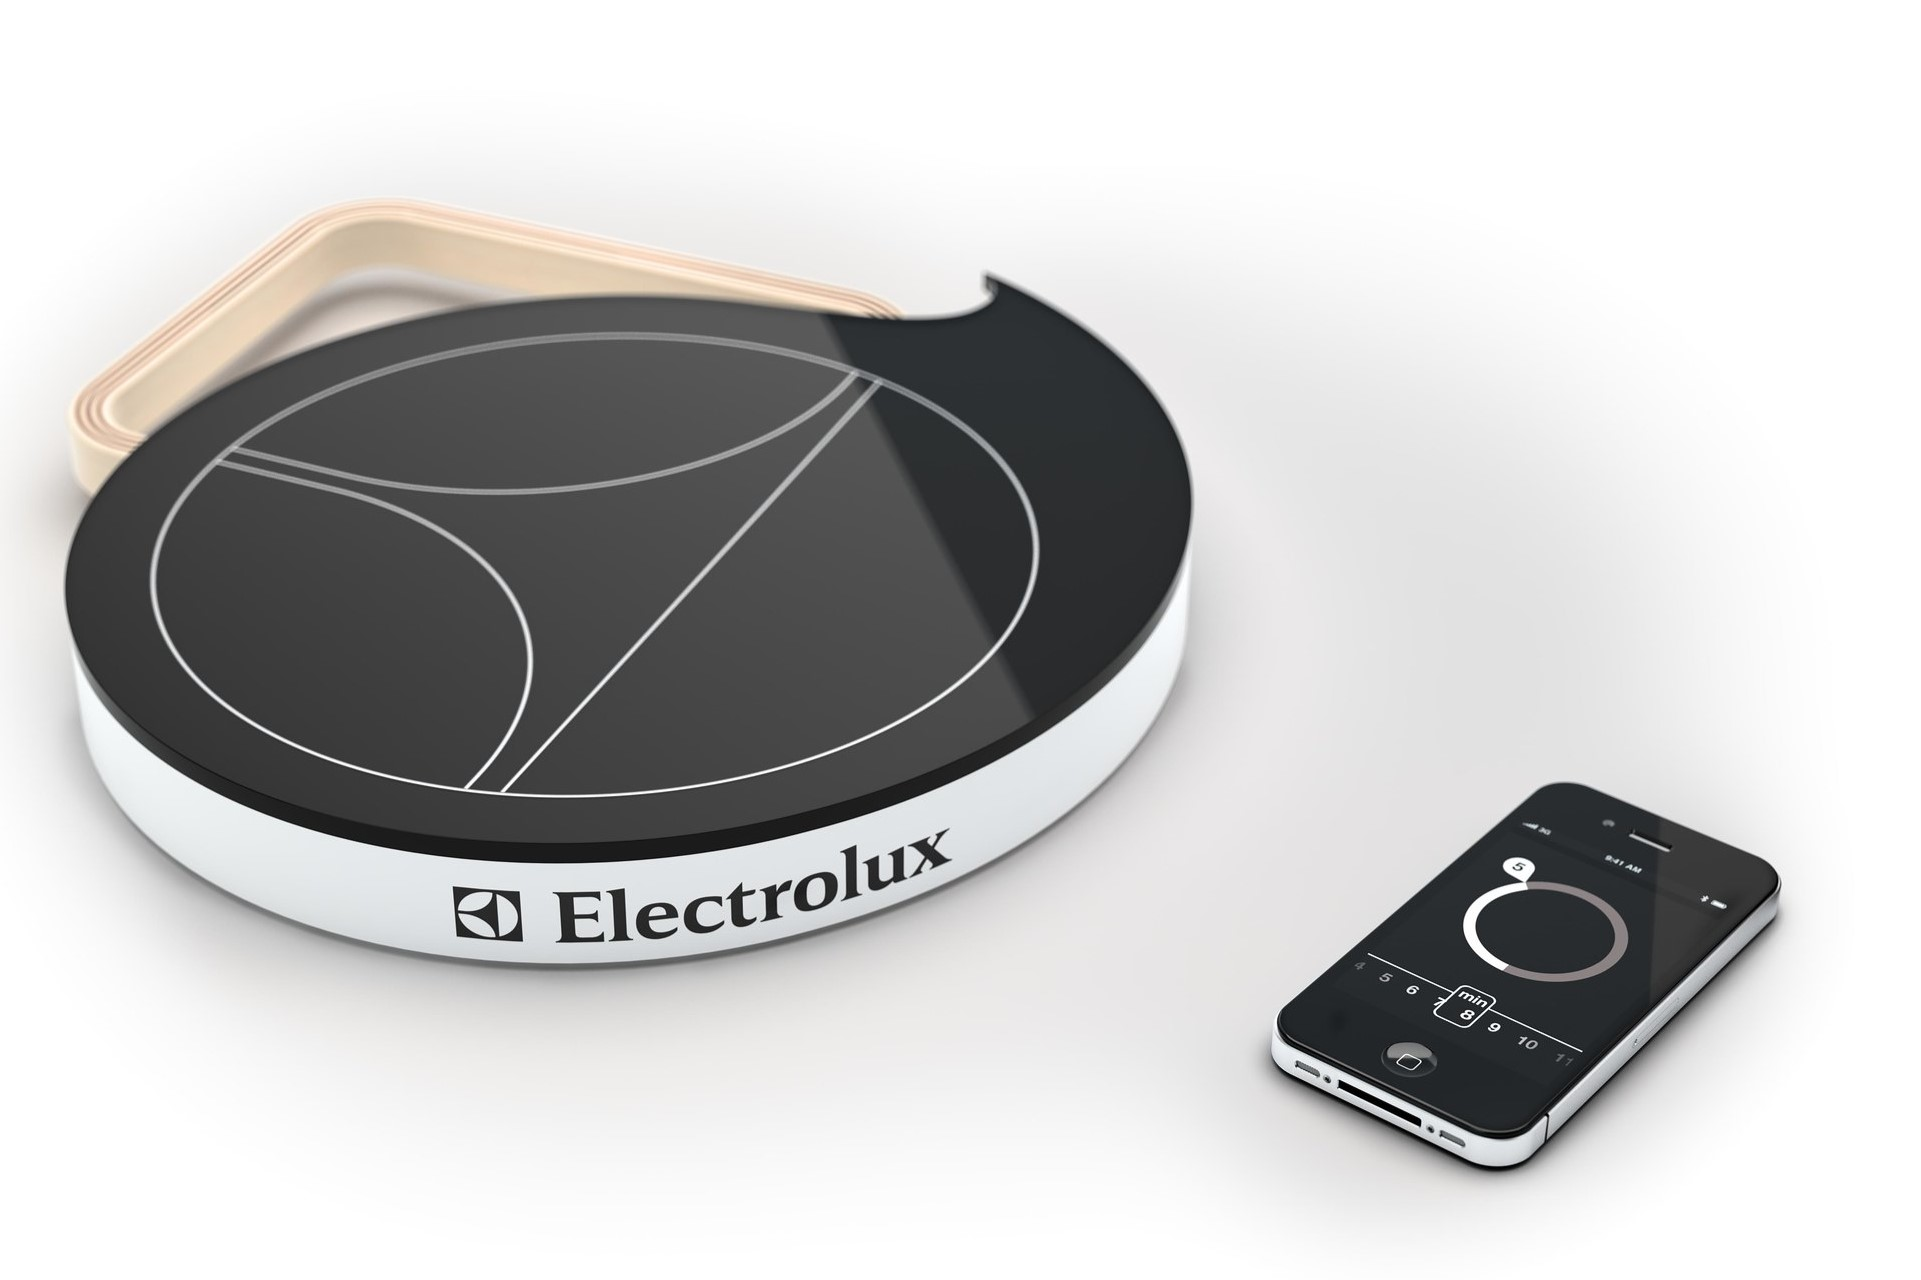
\includegraphics[width=0.5\textwidth]{fig/lec01/Induction_plate.jpg}
			\caption{Induction plate (source: \href{https://www.flickr.com/photos/electrolux-design-lab/6035618944}{flickr}, Electrolux, \href{https://creativecommons.org/licenses/by-nc/2.0/}{CC~BY-SA-NC~2.0})}
		\end{subfigure}
		\hfill
		\begin{subfigure}[b]{0.49\textwidth}
			\centering
			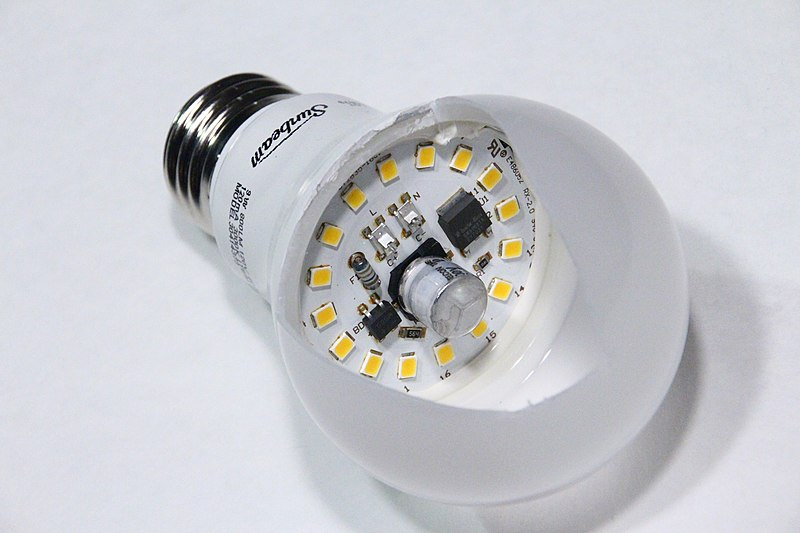
\includegraphics[width=0.5\textwidth]{fig/lec01/LED_light_bulb.jpg}
			\caption{LED rectifier (source: \href{https://commons.wikimedia.org/wiki/File:LED-E27-Light-Bulb-1134.jpg}{Wikimedia Commons}, D.~Tribble, \href{https://creativecommons.org/licenses/by-sa/4.0/deed.en}{CC~BY-SA~4.0})}
		\end{subfigure}
	\end{figure}
\end{frame}

%%%%%%%%%%%%%%%%%%%%%%%%%%%%%%%%%%%%%%%%%%%%%%%%%%%%%%%%%%%%%
%% Power electronic application examples: industrial %%
%%%%%%%%%%%%%%%%%%%%%%%%%%%%%%%%%%%%%%%%%%%%%%%%%%%%%%%%%%%%%
\begin{frame}[c]
	\frametitle{Power electronic application examples: industrial}
	\begin{figure}
		\centering
		\begin{subfigure}[b]{0.49\textwidth}
			\centering
			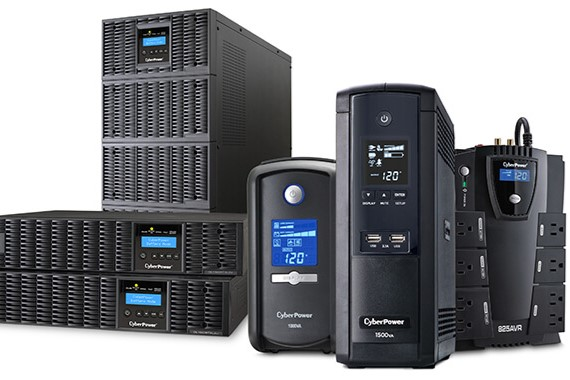
\includegraphics[width=0.5\textwidth]{fig/lec01/UPS.jpg}
			\caption{Uninterruptible power supply (source: \href{https://commons.wikimedia.org/wiki/File:CyberPower_UPS_Systems.jpg}{Wikimedia Commons}, Stevebwallace, \href{https://creativecommons.org/licenses/by-sa/4.0/deed.en}{CC~BY-SA~4.0})}
		\end{subfigure}
		\hfill
		\begin{subfigure}[b]{0.49\textwidth}
			\centering
			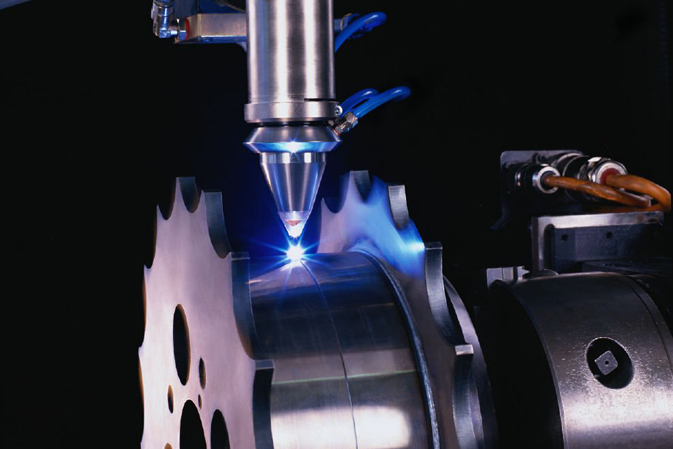
\includegraphics[width=0.5\textwidth]{fig/lec01/Welding.jpg}
			\caption{Welding power supply (source: \href{https://commons.wikimedia.org/wiki/File:Trumpf_laserschweissen.jpg}{Wikimedia Commons}, Trumpf GmbH, \href{https://creativecommons.org/licenses/by-sa/3.0/deed.en}{CC~BY-SA~3.0})}
		\end{subfigure}
		\\
		\begin{subfigure}[b]{0.49\textwidth}
			\centering
			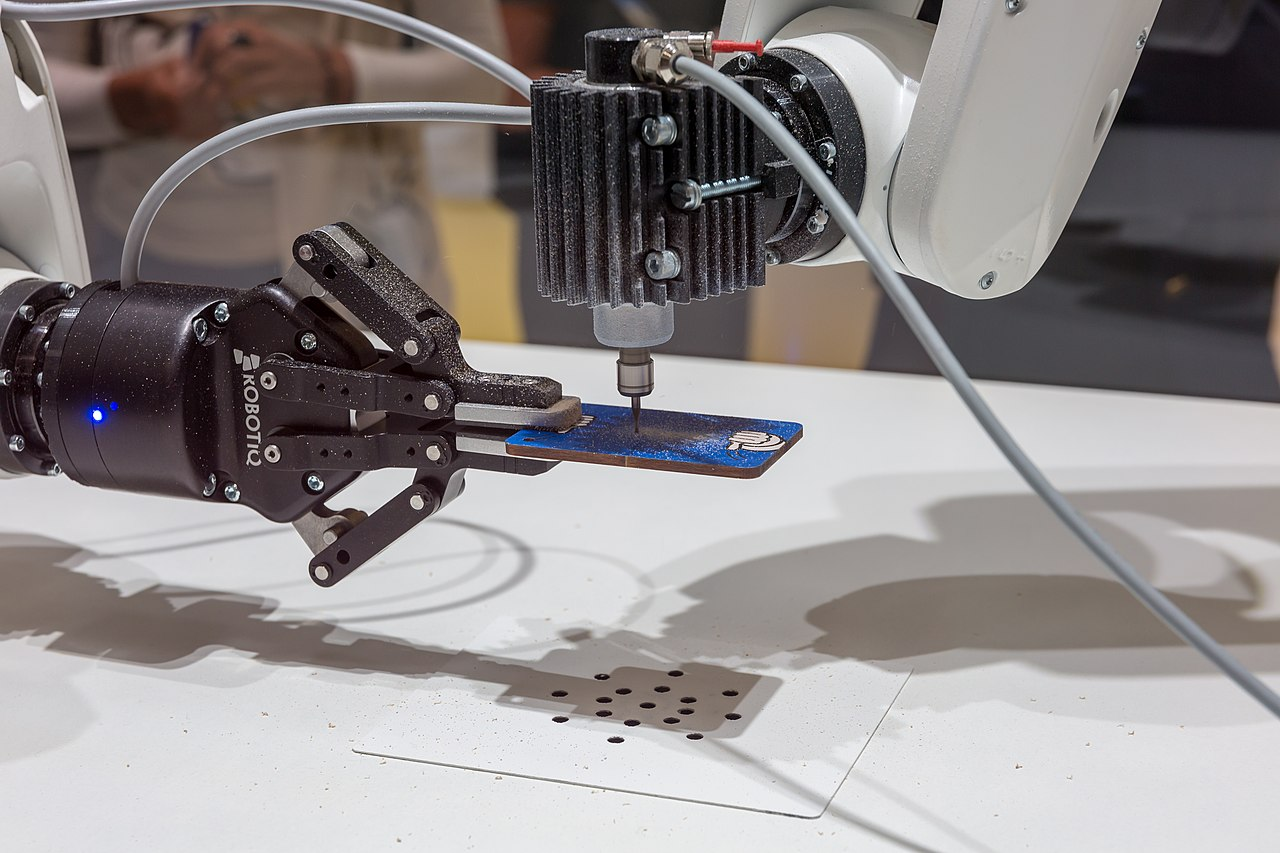
\includegraphics[width=0.5\textwidth]{fig/lec01/Robot.jpg}
			\caption{Industrial drives / automation (source: \href{https://de.m.wikipedia.org/wiki/Datei:Paris_Motor_Show_2018,_Paris_\%281Y7A1752\%29.jpg}{Wikimedia Commons}, M.~BLume, \href{https://creativecommons.org/licenses/by-sa/4.0/deed.de}{CC~BY-SA~4.0})}
		\end{subfigure}
		\hfill
		\begin{subfigure}[b]{0.49\textwidth}
			\centering
			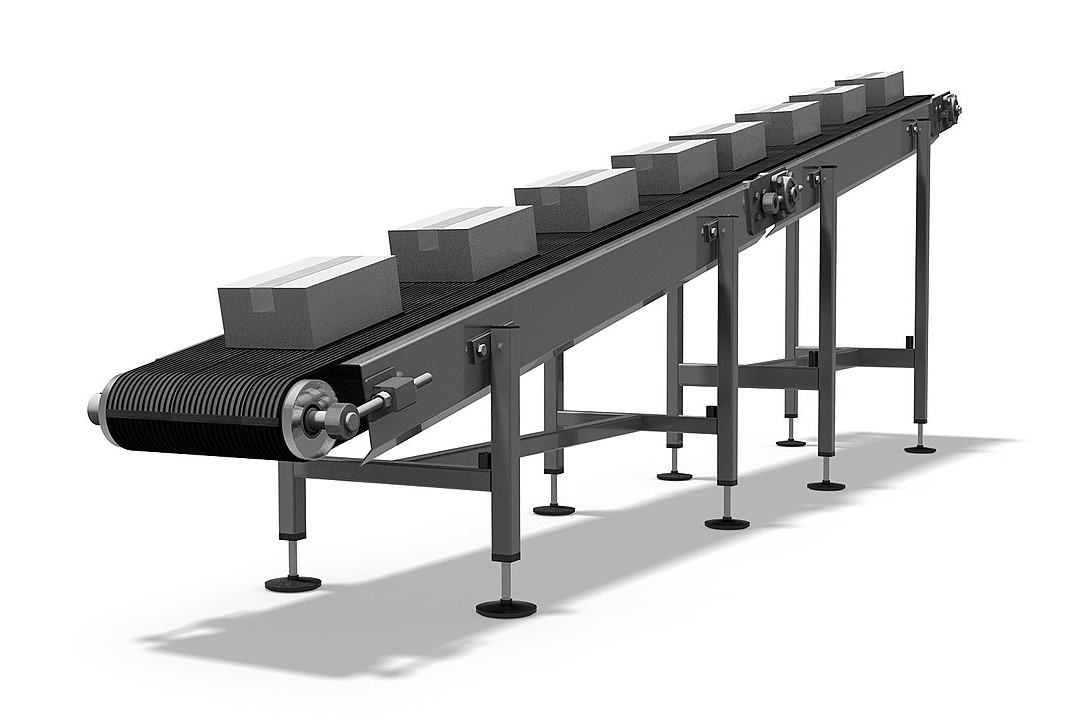
\includegraphics[width=0.5\textwidth]{fig/lec01/Conveyor.jpg}
			\caption{Conveyor belt drive (source: \href{https://commons.wikimedia.org/wiki/File:Inclined-belt_conveyor.jpgg}{Wikimedia Commons},  	K.~Hannessen, \href{https://creativecommons.org/licenses/by-sa/4.0/deed.en}{CC~BY-SA~4.0})}
		\end{subfigure}
	\end{figure}
\end{frame}

%%%%%%%%%%%%%%%%%%%%%%%%%%%%%%%%%%%%%%%%%%%%%%%%%%%%%%%%%%%%%
%% Power electronic application examples: energy system %%
%%%%%%%%%%%%%%%%%%%%%%%%%%%%%%%%%%%%%%%%%%%%%%%%%%%%%%%%%%%%%
\begin{frame}[c]
	\frametitle{Power electronic application examples: energy system}
	\begin{figure}
		\centering
		\begin{subfigure}[b]{0.49\textwidth}
			\centering
			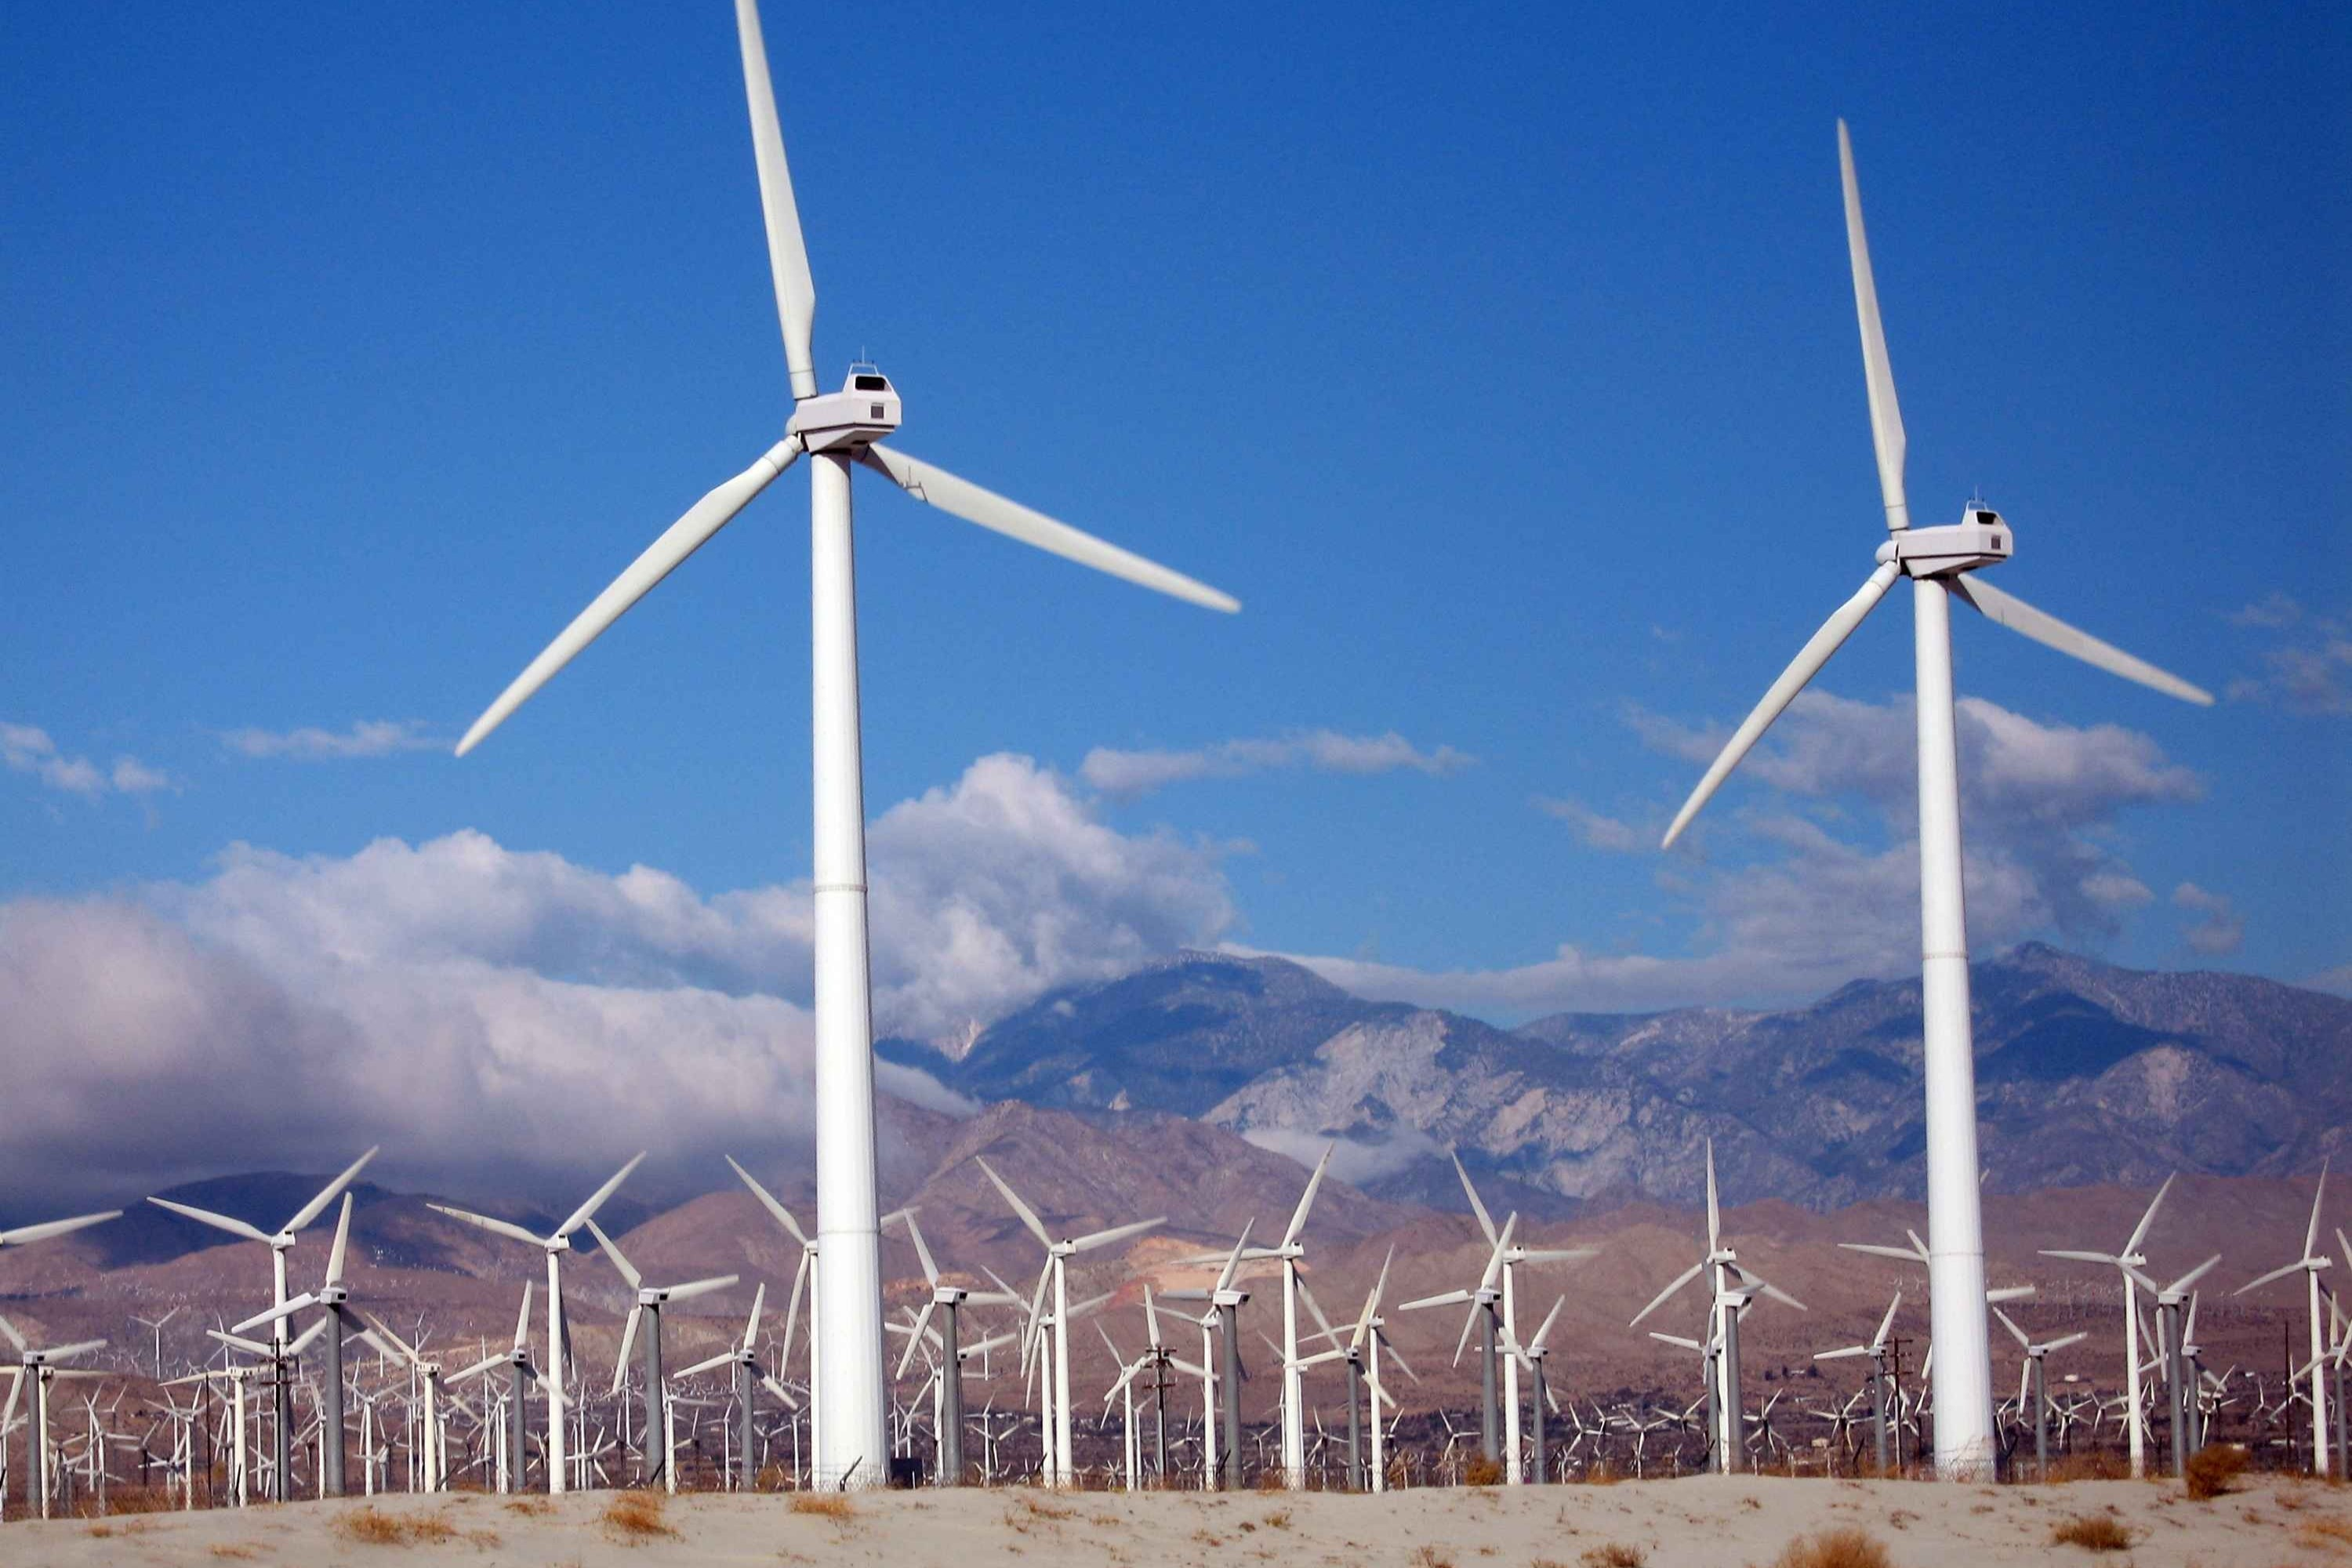
\includegraphics[width=0.5\textwidth]{fig/lec01/sky-farm-windmill.jpg}
			\caption{Wind power plants (source: \href{https://pxhere.com/en/photo/954757}{pxhere}, \href{https://creativecommons.org/publicdomain/zero/1.0/}{CC0~1.0})}
		\end{subfigure}
		\hfill
		\begin{subfigure}[b]{0.49\textwidth}
			\centering
			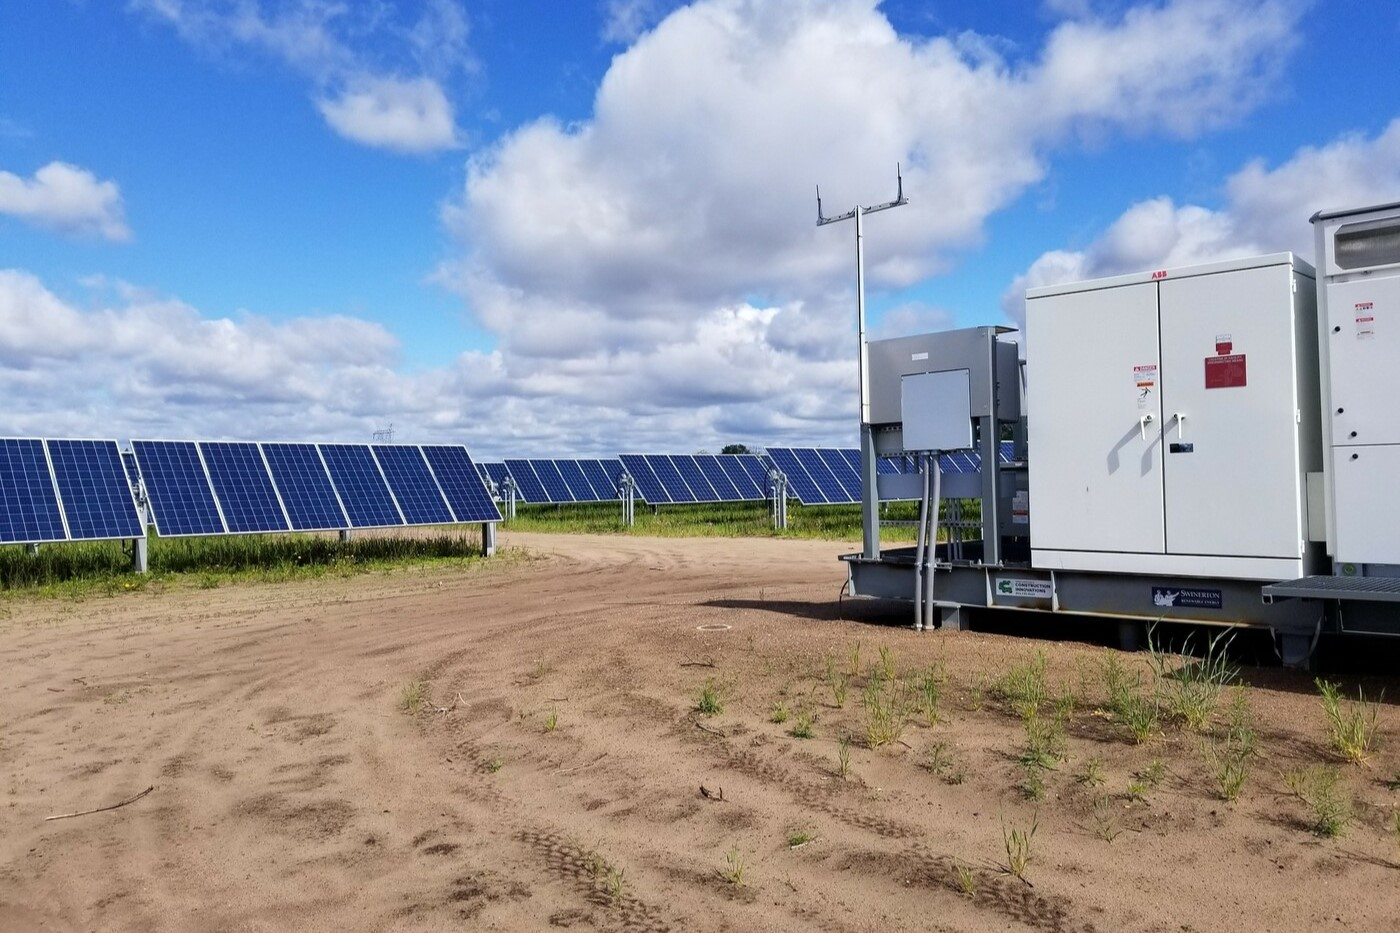
\includegraphics[width=0.5\textwidth]{fig/lec01/PV_field.jpg}
			\caption{PV power plants (source: \href{https://pxhere.com/en/photo/1685464}{pxhere}, \href{https://creativecommons.org/publicdomain/zero/1.0/}{CC0~1.0})}
		\end{subfigure}
		\\
		\begin{subfigure}[b]{0.49\textwidth}
			\centering
			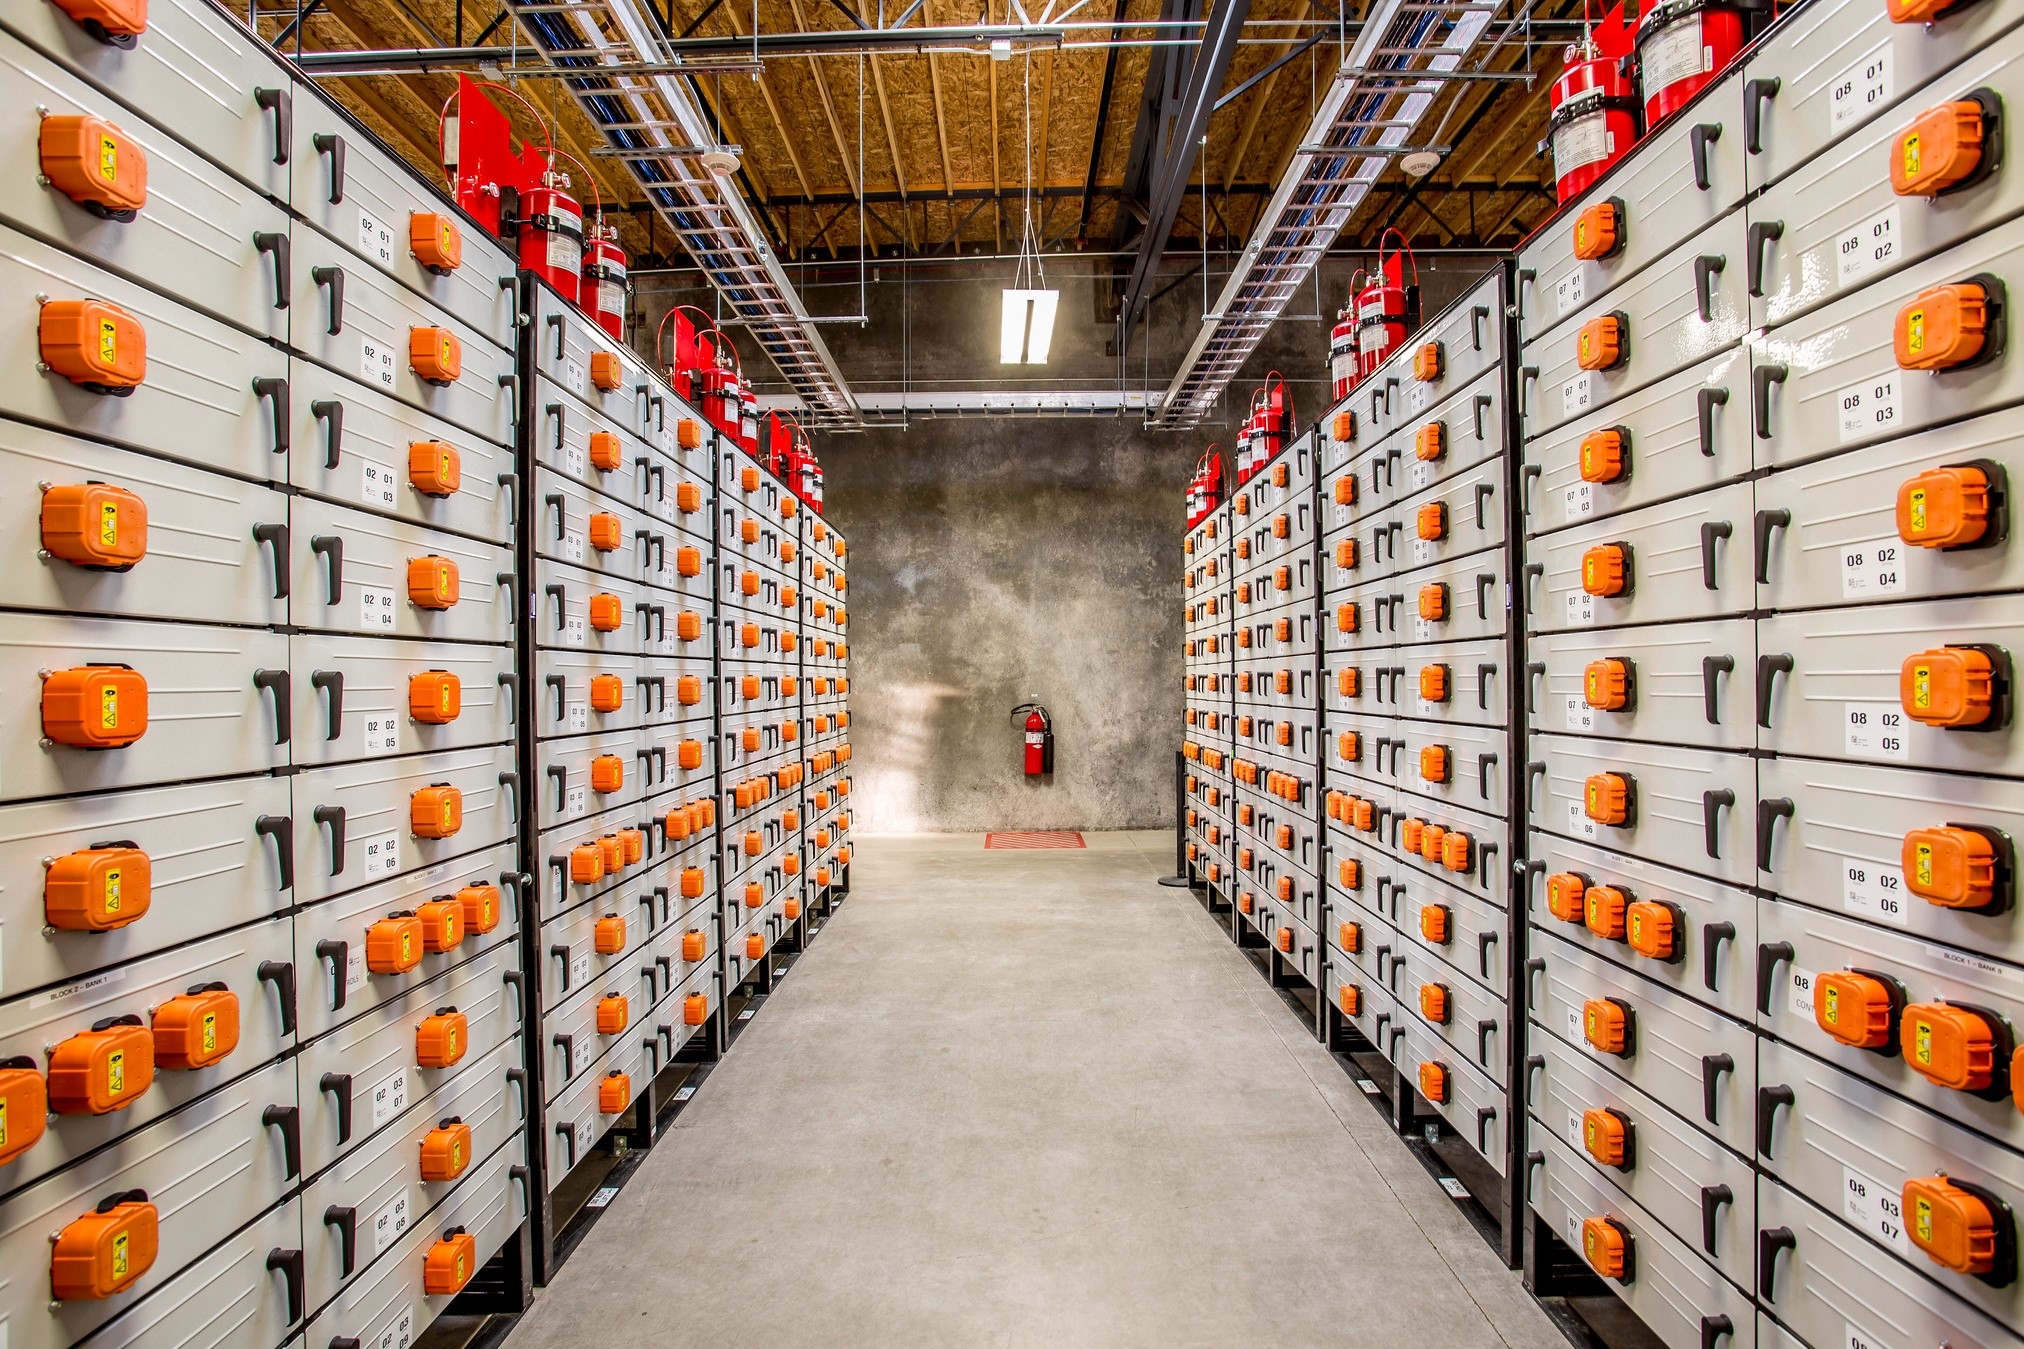
\includegraphics[width=0.5\textwidth]{fig/lec01/Battery_storage.jpg}
			\caption{Battery storage systems (source: \href{https://www.flickr.com/photos/portlandgeneralelectric/8905201835}{flickr}, 
			Portland General Electric, \href{https://creativecommons.org/licenses/by-nd/2.0/}{CC~BY-ND~2.0})}
		\end{subfigure}
		\hfill
		\begin{subfigure}[b]{0.49\textwidth}
			\centering
			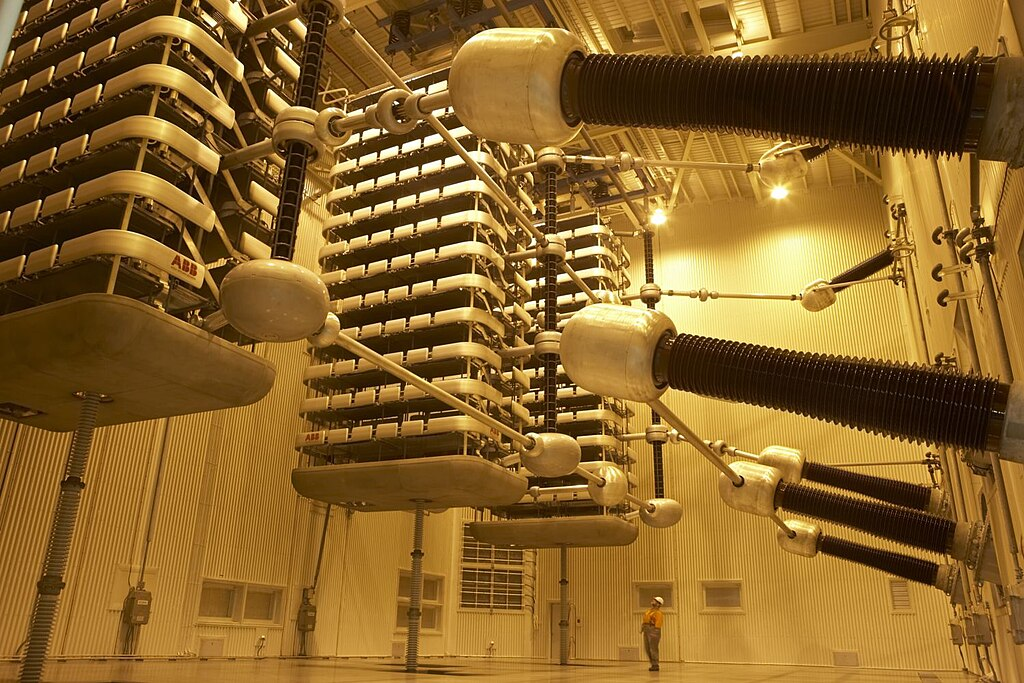
\includegraphics[width=0.5\textwidth]{fig/lec01/HVDC.jpg}
			\caption{High voltage DC transmission (source: \href{https://commons.wikimedia.org/wiki/File:Pole_2_Thyristor_Valve.jpg}{Wikimedia Commons},  	 	Marshelec, \href{https://creativecommons.org/licenses/by-sa/3.0/deed.en}{CC~BY-SA~3.0})}
		\end{subfigure}
	\end{figure}
\end{frame}

%%%%%%%%%%%%%%%%%%%%%%%%%%%%%%%%%%%%%%%%%%%%%%%%%%%%%%%%%%%%%
%% Power electronic application examples: transportation %%
%%%%%%%%%%%%%%%%%%%%%%%%%%%%%%%%%%%%%%%%%%%%%%%%%%%%%%%%%%%%%
\begin{frame}[c]
	\frametitle{Power electronic application examples: transportation}
	\begin{figure}
		\centering
		\begin{subfigure}[b]{0.49\textwidth}
			\centering
			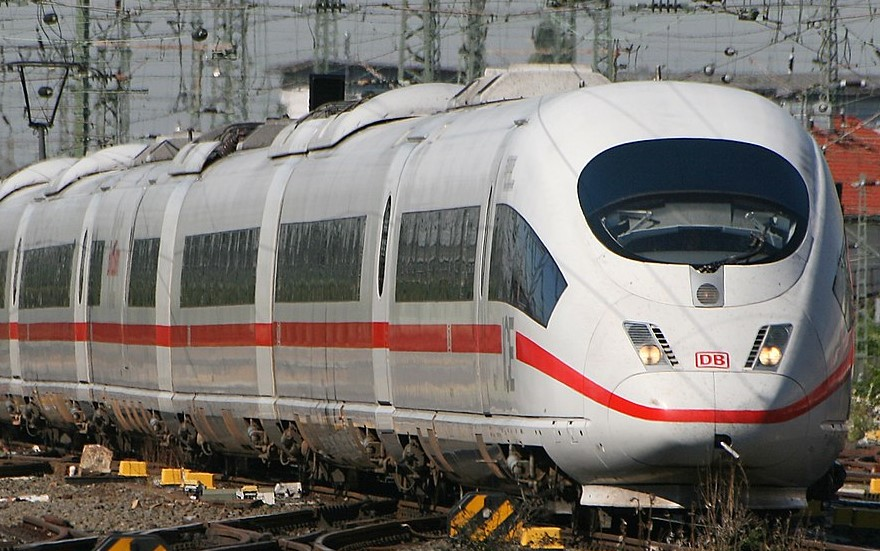
\includegraphics[width=0.5\textwidth]{fig/lec01/ICE.jpg}
			\caption{Train drive (source: \href{hhttps://commons.wikimedia.org/wiki/File:DB_AG_406_001-8.jpg}{Wikimedia Commons}, T.~Wolf, \href{https://creativecommons.org/publicdomain/zero/1.0/}{CC0~1.0})}
		\end{subfigure}
		\hfill
		\begin{subfigure}[b]{0.49\textwidth}
			\centering
			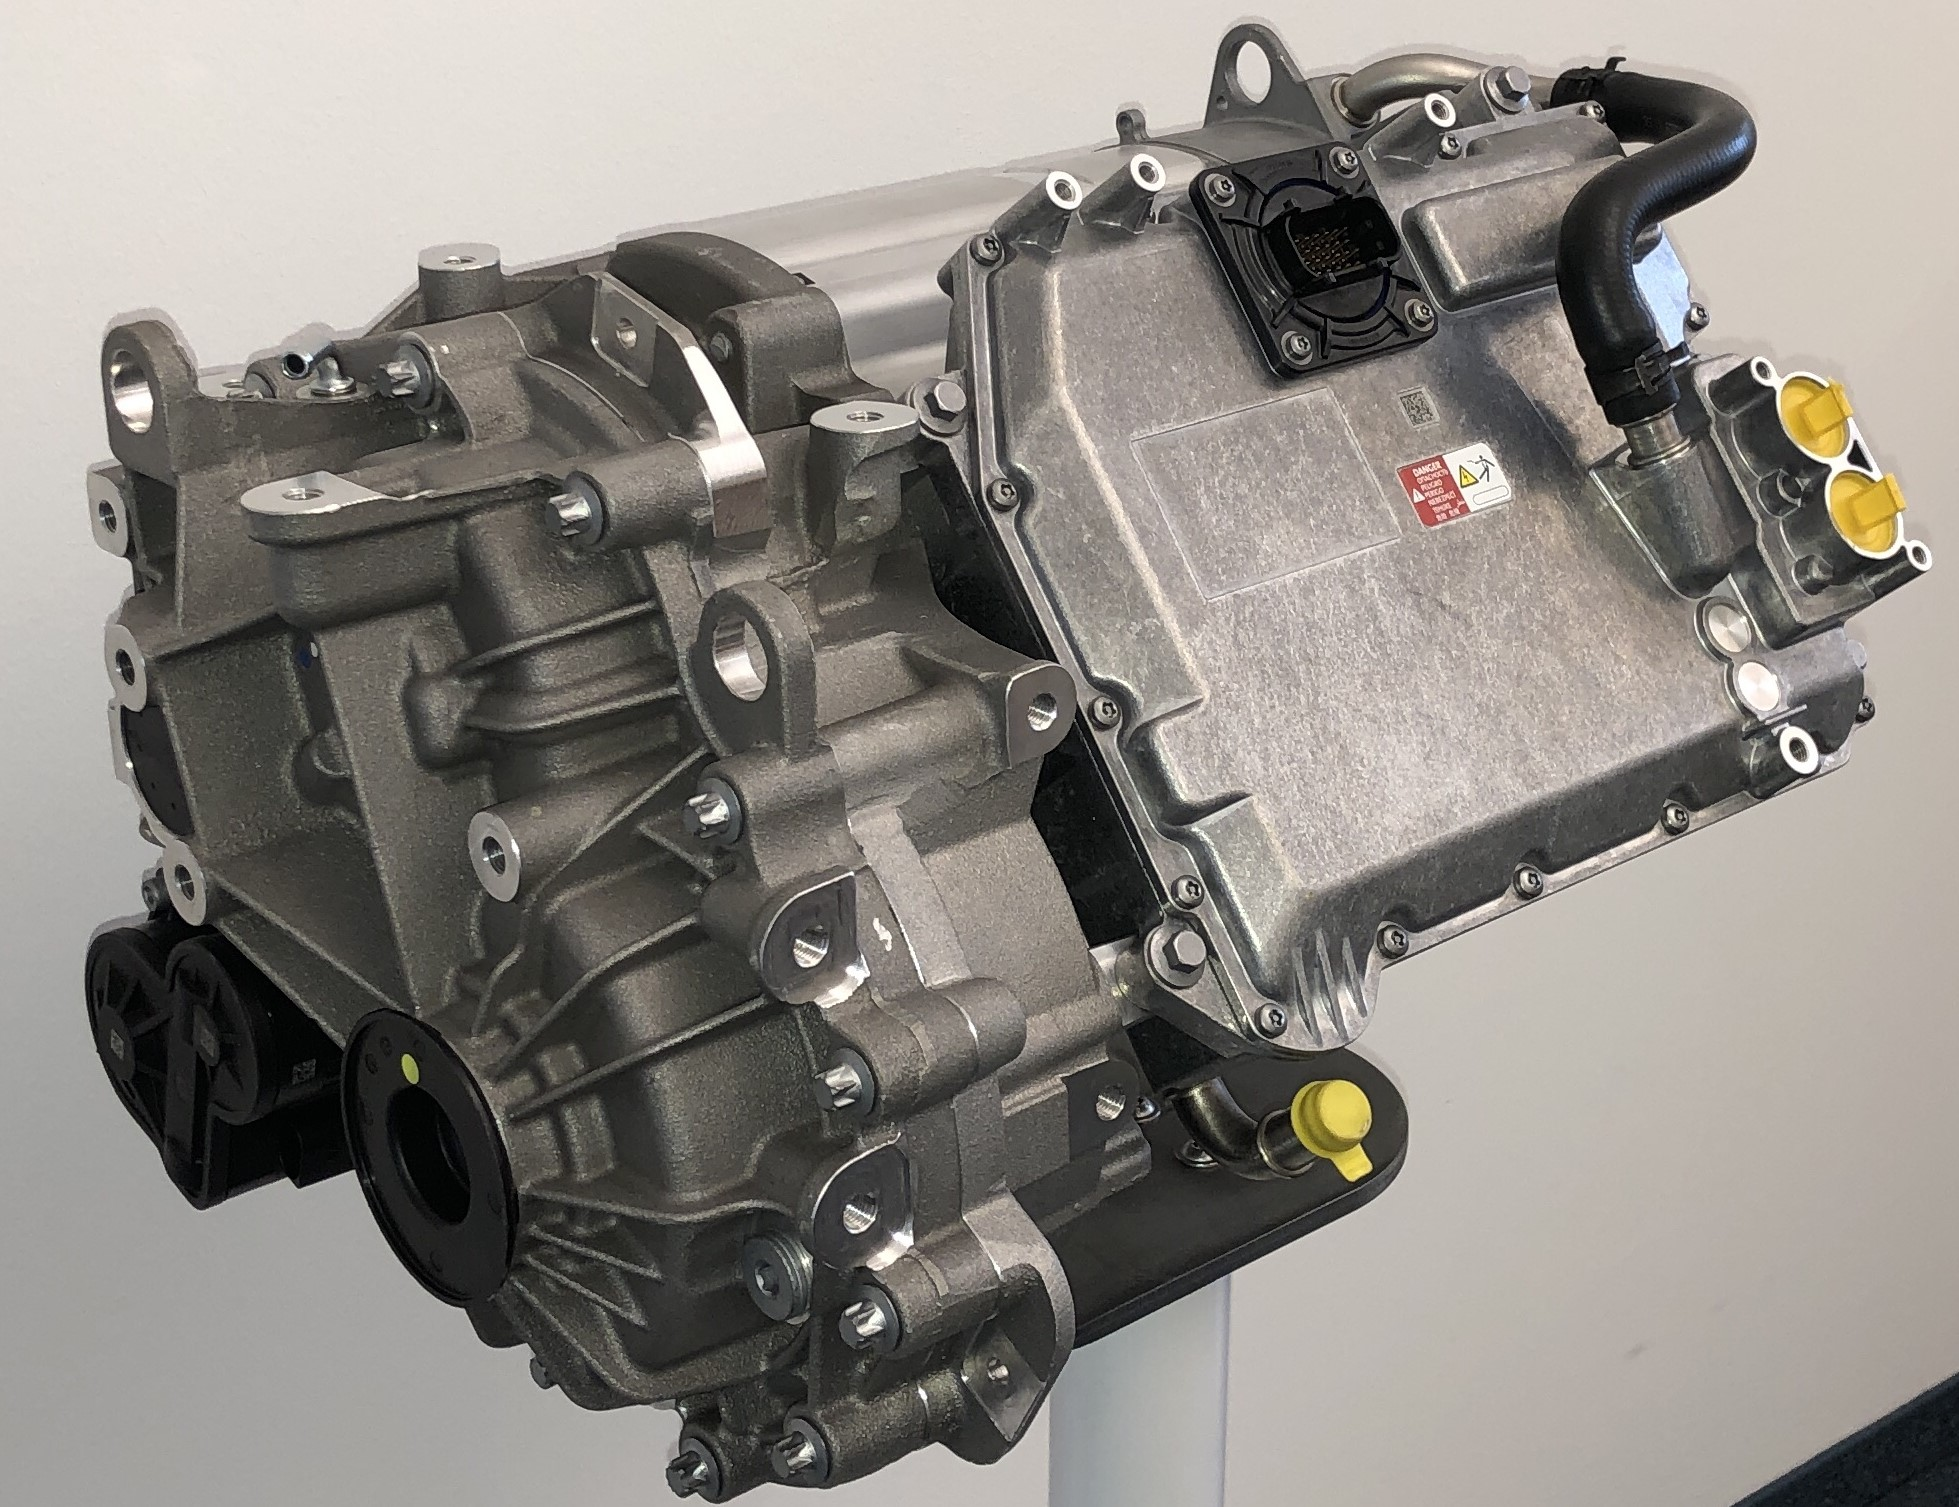
\includegraphics[width=0.5\textwidth]{fig/lec01/Drive.jpg}
			\caption{Electric vehicle drive (source: \href{https://commons.wikimedia.org/wiki/File:Vitesco_Technologies_EMR3.jpg}{Wikimedia Commons}, Caprolactam123, \href{https://creativecommons.org/licenses/by-sa/4.0/deed.en}{CC~BY-SA~4.0})}
		\end{subfigure}
		\\
		\begin{subfigure}[b]{0.49\textwidth}
			\centering
			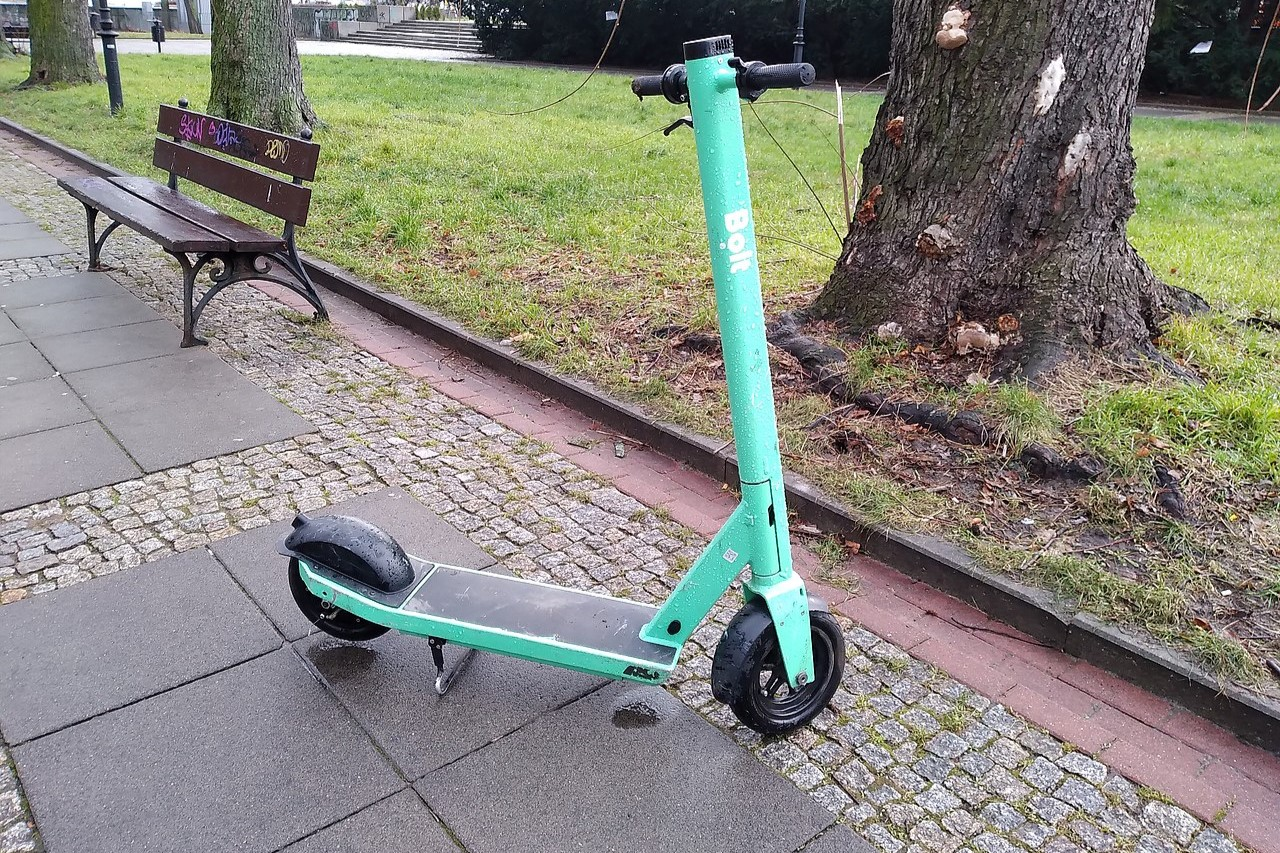
\includegraphics[width=0.5\textwidth]{fig/lec01/Scooter.jpg}
			\caption{Electric scooter (source: \href{https://commons.wikimedia.org/wiki/File:Bolt_Electric_Scooter_\%28Warsaw\%29_in_2020.03.jpg}{Wikimedia Commons}, Raju, \href{https://creativecommons.org/licenses/by-sa/4.0/deed.en}{CC~BY-SA~4.0})}
		\end{subfigure}
		\hfill
		\begin{subfigure}[b]{0.49\textwidth}
			\centering
			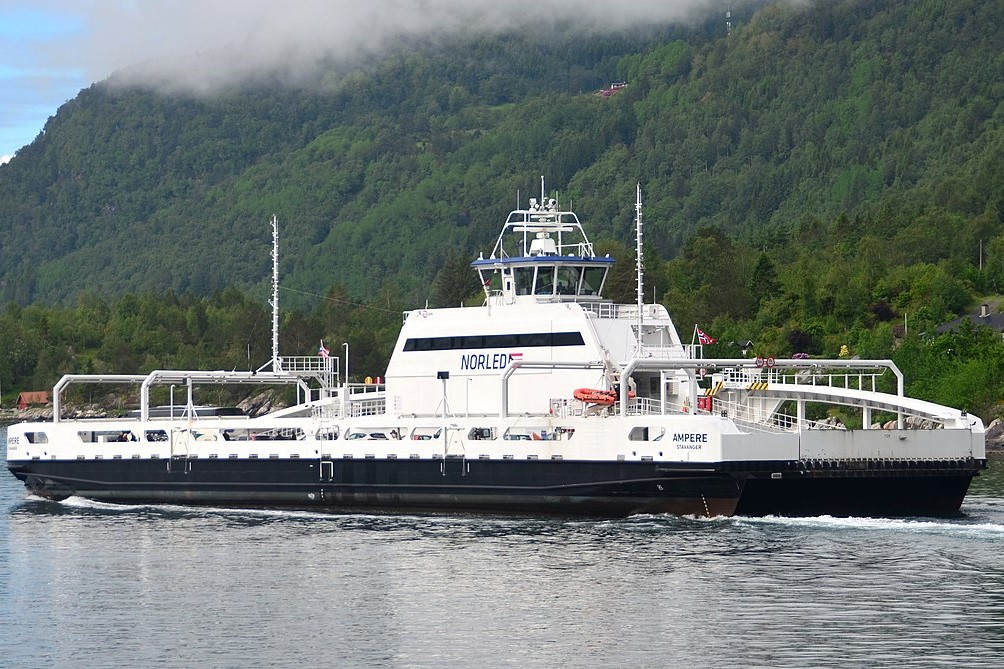
\includegraphics[width=0.5\textwidth]{fig/lec01/Electric_ship.jpg}
			\caption{Electic ship (source: \href{https://commons.wikimedia.org/wiki/File:Ferry_Ampere_Sognefjord.jpg}{Wikimedia Commons},  	 	Wikimalte, \href{https://creativecommons.org/licenses/by-sa/4.0/deed.en}{CC~BY-SA~4.0})}
		\end{subfigure}
	\end{figure}
\end{frame}

%%%%%%%%%%%%%%%%%%%%%%%%%%%%%%%%%%%%%%%%%%%%%%%%%%%%%%%%%%%%%
%% A broad range of nominal power ratings %%
%%%%%%%%%%%%%%%%%%%%%%%%%%%%%%%%%%%%%%%%%%%%%%%%%%%%%%%%%%%%%
\begin{frame}[c]
	\frametitle{A broad range of nominal power ratings}
	\vspace{0.3cm}
	\begin{figure}
		\centering
		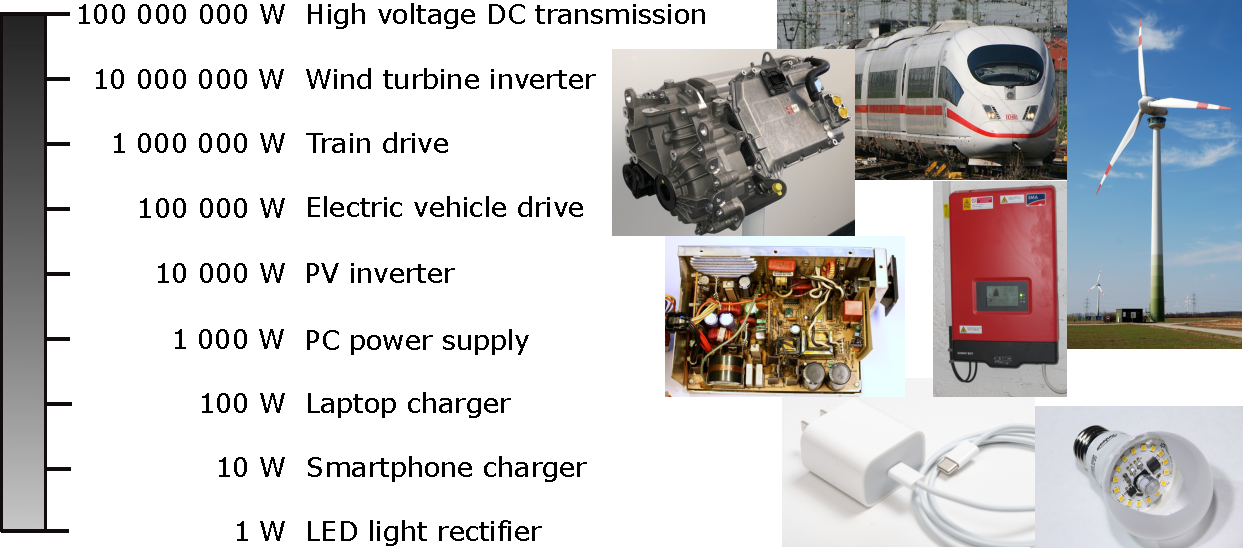
\includegraphics[height=0.7\textheight]{fig/lec01/Power_Classes_Examples.pdf}
		\caption{Power range overview (figure sources: \href{https://commons.wikimedia.org/wiki/File:DB_AG_406_001-8.jpg}{T. Wolf}, \href{https://commons.wikimedia.org/wiki/File:Wind_turbine_with_observation_deck_bruck_an_der_leitha.jpg}{KoeppiK}, \href{https://commons.wikimedia.org/wiki/File:Vitesco_Technologies_EMR3.jpg}{Caprolactam123}, \href{https://commons.wikimedia.org/wiki/File:Installation_of_solar_PV_panels_-_inverter_-_geograph.org.uk_-_2624304.jpg}{D. Hawgood}, \href{https://commons.wikimedia.org/wiki/File:IBM_PC_XT_5160_Power_Supply.jpg}{Mister rf}, \href{https://commons.wikimedia.org/wiki/File:LED-E27-Light-Bulb-1134.jpg}{D.~Tribble} and \href{https://www.rawpixel.com/image/5923136/photo-image-phone-public-domain-white}{rawpixel} under varying CC licenses) }
		\label{Power_Classes_Examples}
	\end{figure}
\end{frame}

%%%%%%%%%%%%%%%%%%%%%%%%%%%%%%%%%%%%%%%%%%%%%%%%%%%%%%%%%%%%%
%% Terminology: work vs. energy%%
%%%%%%%%%%%%%%%%%%%%%%%%%%%%%%%%%%%%%%%%%%%%%%%%%%%%%%%%%%%%%
\begin{frame}[c]
	\frametitle{Terminology: work vs. energy}
	\begin{columns}
		\begin{column}{0.5\textwidth}
			\begin{varblock}{Work}
				Work is the integral of the power over a time integral (or force over distance) and is a measure of the energy transfer.
			\end{varblock}
		\end{column}
		\begin{column}{0.5\textwidth}
			\begin{varblock}{Energy}
				Energy is the capacity to do work, that is, a quantity depending on the state of a system at a given point of time.				
			\end{varblock}
		\end{column}
	\end{columns}
	\vspace{0.5cm}
	\begin{figure}
		\begin{tikzpicture}
			\node[draw, bubble, minimum width = 8em, minimum height = 5em] (energy) at (0,0) {\large Energy};
			\coordinate (loss) at (4.5,-1.25);
			\node[draw, bubble] (energy2) at (6,0) {\large Energy};
			\begin{scope}[on background layer]
				\draw[-{Latex[length=4mm, width=8mm]}, line width=4mm] (energy.mid) -- node[above, midway, name = work] {Work} (energy2);
				\draw[-{Latex[length=4mm, width=8mm]}, line width=2mm, color=signalred, transform canvas={yshift=-3mm}] (energy.mid) --  (3,0) to [out=0,in=120] (loss.south) ;
				\node[below, transform canvas={yshift=-3mm}] at (loss) {\color{signalred} \large Heat};
				\node[below=of work, yshift = 6mm, color=signalred] {Losses};
			\end{scope}
		\end{tikzpicture}
		\vspace{0.75cm}
		\caption{Illustration addressing the work vs. energy terminology (simplified Sankey diagram)}
		\label{fig:work_vs_energy}
	\end{figure}
\end{frame}

%%%%%%%%%%%%%%%%%%%%%%%%%%%%%%%%%%%%%%%%%%%%%%%%%%%%%%%%%%%%%
%% Power Power balance of an electrical energy conversion system %%
%%%%%%%%%%%%%%%%%%%%%%%%%%%%%%%%%%%%%%%%%%%%%%%%%%%%%%%%%%%%%
\begin{frame}
	\frametitle{Power balance of an electrical energy conversion system}
	\begin{figure}
		\begin{tikzpicture}[auto, node distance = 1.5cm and 2cm]
			\draw
				node [input, name = input] {}
				node [bubble, right = of input, minimum height = 4em, pin=80:Change of stored energy $ \frac{\mathrm{d}}{\mathrm{d}t}E_\mathrm{i}(t)$] (pc) {\large Power converter}
				node [output, name = output, right = of pc] {}
				node [output, name = losses, below = of pc] {};
			\draw[-{Latex[length=4mm, width=8mm]}, line width=3mm] (input) -- node[below, midway, align=left, name = input2] {Electrical\\input power} (pc);
			\begin{scope}[on background layer]
				\draw[-{Latex[length=4mm, width=8mm]}, line width=3mm] (pc.mid) -- node[below, near end, align=left, name=output2] {Electrical\\output power} (output);
				\draw[-{Latex[length=4mm, width=8mm]}, line width=3mm, color=signalred] (pc.mid) -- node[right, yshift=-2.5mm, name = losses2] {Losses} (losses);
			\end{scope}
			\node[left=of losses2, color=signalred, xshift = 1.8cm] {$P_\mathrm{l}(t)$};
			\node[above=of output2.mid,, align=center, xshift = -0.3cm, yshift = -5mm] {$P_\mathrm{out}(t)$};
			\node[above=of input2.mid,, align=center, xshift = -0.3cm, yshift = -5mm] {$P_\mathrm{in}(t)$};
		\end{tikzpicture}
		\caption{Power balance of an energy conversion system}
		\label{fig:power_balance_energy_conversion}
	\end{figure}
	\vspace{-0.5cm}
	The power balance
	\begin{equation}
		P_\mathrm{in}(t) = P_\mathrm{out}(t) + P_\mathrm{l}(t) + \frac{\mathrm{d}}{\mathrm{d}t}E_\mathrm{i}(t)
	\end{equation}
	must hold for any point in time as energy is conserved, that is, not created or destroyed.
\end{frame}

%%%%%%%%%%%%%%%%%%%%%%%%%%%%%%%%%%%%%%%%%%%%%%%%%%%%%%%%%%%%%
%% Why efficiency matters: a computer supply example %%
%%%%%%%%%%%%%%%%%%%%%%%%%%%%%%%%%%%%%%%%%%%%%%%%%%%%%%%%%%%%%
\begin{frame}[c]
	\frametitle{Why efficiency matters: a computer supply example}
	\begin{table}
		\centering
		\begin{tabular}{lcc}
			\toprule
			& Power supply A & Power supply B \\
			& 80 PLUS Gold & 80 PLUS Titanium \\
			\midrule
			Input power & \multicolumn{2}{c}{\SI{250}{\watt}} \\
			Efficiency & \SI{89}{\percent} & \SI{94}{\percent}  \\
			Power loss & \SI{27.5}{\watt} & \SI{15}{\watt}\\
			\midrule
			Operating hours per year & \multicolumn{2}{c}{$\SI{8}{\hour} \times 220 = \SI{1760}{\hour}$} \\
			Cumulated power loss per year & \SI{48.4}{\kilo\watt\hour} & \SI{26.4}{\kilo\watt\hour} \\
			Electricity cost for yearly power losses & \SI{14.52}{\EUR} & \SI{7.92}{\EUR} \\
			\midrule
			Cumulated power loss in Germany & \SI{1.936}{\tera\watt\hour} & \SI{1.056}{\tera\watt\hour} \\
			Electricity cost for power loss in Germany & \SI{580.8}{\mega\EUR} & \SI{316.8}{\mega\EUR} \\
			\bottomrule
		\end{tabular}
		\label{tab:efficiency_computer_supply_example}
		\caption{Comparison of two computer power supplies (further assumptions: effective nominal power calculation, electricity price \SI[fraction-function=\nicefrac]{0.3}{\EUR\per\kilo\watt\per\hour}, $40\cdot 10^6$ computers in Germany)}
	\end{table}
\end{frame}

%%%%%%%%%%%%%%%%%%%%%%%%%%%%%%%%%%%%%%%%%%%%%%%%%%%%%%%%%%%%%
%% Why efficiency matters: a wind power plant example %%
%%%%%%%%%%%%%%%%%%%%%%%%%%%%%%%%%%%%%%%%%%%%%%%%%%%%%%%%%%%%%
\begin{frame}[c]
	\frametitle{Why efficiency matters: a wind power plant example}
	\begin{table}
		\centering
		\begin{tabular}{lcc}
			\toprule
			& Wind power plant A & Wind power plant B \\
			\midrule
			Input power & \multicolumn{2}{c}{\SI{5}{\mega\watt}} \\
			Efficiency & \SI{97}{\percent} & \SI{97.1}{\percent}  \\
			Power loss & \SI{150}{\kilo\watt} & \SI{145}{\kilo\watt}\\
			\midrule
			Nominal power operating hours per year & \multicolumn{2}{c}{$\SI{3000}{\hour}$} \\
			Cumulated power loss per year & \SI{450}{\mega\watt\hour} & \SI{435}{\mega\watt\hour} \\
			Cumulated power loss (lifetime) & \SI{9.0}{\giga\watt\hour} & \SI{8.7}{\giga\watt\hour} \\
			\midrule
			Lost sales proceeds due to losses per year  & \SI{22.5}{\kilo\EUR} & \SI{21.75}{\kilo\EUR} \\
			Lost sales proceeds due to losses (lifetime)  & \SI{450}{\kilo\EUR} & \SI{435}{\kilo\EUR} \\
			\midrule
			Cumulated power loss (lifetime, Germany)  & \SI{9.0}{\tera\watt\hour} & \SI{8.7}{\tera\watt\hour} \\
			Lost sales proceeds (lifetime, Germany)  & \SI{450}{\mega\EUR} & \SI{435}{\mega\EUR} \\
			\bottomrule
		\end{tabular}
		\label{tab:efficiency_wind_power_example}
		\caption{Comparison of two wind power plants (further assumptions:  electricity sales price \SI[fraction-function=\nicefrac]{0.05}{\EUR\per\kilo\watt\per\hour}, $20$ years of life time, $\num{1000}$ newly constructed wind power plants per year in Germany)}
	\end{table}
\end{frame}